% \chapter{Results and Publications}

% \section{Evaluation Matrix}
% \subsubsection*{Root Mean Squared Error (RMSE)}
% On this basis, the Root Mean Squared Error (RMSE) is an evaluation criterion with reference to the accuracy of the model’s forecast. It is actually the square root of the arithmetic mean of the squared difference between them and the predicted values. RMSE offers further information to do with unequal trifling with the scale of data especially for regression models, in circumstance of absolute mistakes. It is defined as follows:

% \begin{equation}
% \text{RMSE} = \sqrt{\frac{1}{n} \sum_{i=1}^{n} (y_i - \hat{y}_i)^2}
% \end{equation}

% where:
% \begin{itemize}
%     \item \( n \) is the number of observations,
%     \item \( y_i \) is the actual value of the \(i^{th}\)observation,
%     \item \( \hat{y}_i \) is the predicted value of the \(i^{th}\) observation.
% \end{itemize}

% \subsubsection*{R-squared (R²)}
% The coefficient of multiple determination R² is an R statistic the measures percentage or proportion of variance in the dependent/forecasted variable, explained by the changes in one or organisms independent/predictor variable. It helps us to know how well the regression model has been fitted into the data. The Squared Multiple Correlation values has a range of 0 – 1 where the value of 1 mean all variations have been explained by the model while the value 0 means no variation in the data has been explained by the model. Another measure of the reliability of the model can also be estimate from the statistic R² whereby a higher value is preferred. It is
% defined as follows:

% \begin{equation}
% R^2 = 1 - \frac{\sum_{i=1}^{n} (y_i - \hat{y}_i)^2}{\sum_{i=1}^{n} (y_i - \bar{y})^2}
% \end{equation}

% where:
% \begin{itemize}
%     \item \( n \) stands the number of observations,
%     \item \( y_i \) stands for the true value the \(i^{th}\) observation,
%     \item \( \hat{y}_i \) stands the predicted value of the \(i^{th}\) observation,
%     \item \( \bar{y} \) stands the mean of the actual values.
% \end{itemize}

% \section{Enhanced Hybrid LSTM-RLS Architecture Results}


% Figure \ref{fig:refinedApproachRes1} and \ref{fig:refinedApproachRes2} brings out the performance of the model in terms of identifying the patterns during training, which is reflected in the high R² score.

% % Modify figure sizes according to your needs
% \begin{figure}[h!]
%     \centering
%     \includegraphics[width=\textwidth]{23MAI004_Sem3_MidSem_Report/ActvsPred.pdf}
%     \caption{ Original vs. Predicted Stock Prices }
%     \label{fig:refinedApproachRes1}
% \end{figure}

% \begin{figure}[h!]
%     \centering
%     \includegraphics[width=\textwidth]{23MAI004_Sem3_MidSem_Report/returns_comparision.pdf}
%     \caption{ Returns: Original vs. Predicted Prices }
%     \label{fig:refinedApproachRes2}
% \end{figure}

% Table \ref{tab:lstm_rls_performance} and Table \ref{tab:bi_lstm_rls_performance} show the results of the Hybrid LSTM-RLS model (both LSTM and Bi-LSTM) when the architecture is tested on the test data. The results include RMSE for daily close prices and RMSE when both actual and predicted values are converted into returns, and then the RMSE is calculated between them.

% \begin{table}[h!]
% \centering
% \begin{tabular}{|l|c|c|c|}
% \hline
% \textbf{LSTM-RLS}  & \textbf{Daily Returns} & \textbf{Weekly Returns} & \textbf{Daily Close} \\ \hline
% \textbf{RMSE}      & 0.76\%                 & 1.44\%                 & 161.8935             \\ \hline
% \textbf{R2}        & -0.0636                & -0.038                 & 0.9956               \\ \hline
% \end{tabular}
% \caption{LSTM-RLS Performance Metrics}
% \label{tab:lstm_rls_performance}
% \end{table}

% \begin{table}[h!]
% \centering
% \begin{tabular}{|l|c|c|c|}
% \hline
% \textbf{\textit{Bi-LSTM - RLS}} & \textbf{Daily Returns} & \textbf{Weekly Returns} & \textbf{Daily Close} \\ \hline
% \textbf{RMSE}                   & 0.77\%                 & 2.22\%                 & 161.7337             \\ \hline
% \textbf{R2}                     & -0.0879                & -1.4785                & 0.9956               \\ \hline
% \end{tabular}
% \caption{Bi-LSTM - RLS Performance Metrics}
% \label{tab:bi_lstm_rls_performance}
% \end{table}

% \section{Results with Shift}

% Figures~\ref{fig:revisedApproachshift1} and \ref{fig:revisedApproachshift2} represent the actual daily close versus shifted predicted daily close, and returns calculated on actual daily close versus returns calculated on shifted predicted daily close, respectively.

% % Modify figure sizes according to your needs
% \begin{figure}[h!]
%     \centering
%     \includegraphics[width=\textwidth]{23MAI004_Sem3_MidSem_Report/ActvsPredshift.pdf}
%     \caption{ Stock Prices: Shifted Predictions (-1)}
%     \label{fig:revisedApproachshift1}
% \end{figure}

% \begin{figure}[h!]
%     \centering
%     \includegraphics[width=\textwidth]{23MAI004_Sem3_MidSem_Report/returns_comparisionshift.pdf}
%     \caption{  Returns: Shifted Predictions (-1)}
%     \label{fig:revisedApproachshift2}
% \end{figure}

% Table~\ref{tab:lstm_rls_shift} shows the RMSE comparison between Hybrid LSTM-RLS predicted daily close-based calculated returns and Hybrid LSTM-RLS predicted shifted daily close-based calculated returns.

% \begin{table}[ht]
% \centering
% \begin{tabular}{|l|c|}
% \hline
% \multicolumn{2}{|c|}{\textbf{LSTM-RLS Error between Actual and Predicted Daily Returns}} \\ \hline
% \textbf{Original RMSE}       & 1.01\%   \\ \hline
% \textbf{RMSE with Shift - 1} & \textbf{0.24\%} \\ \hline
% \end{tabular}
% \caption{RMSE Comparison for Daily Returns (LSTM-RLS)}
% \label{tab:lstm_rls_shift}
% \end{table}

% \section{DNS Architecture Results}

% Figure~\ref{fig:DNSplot} shows the best actual vs predicted plot when trained and tested on the DNS architecture to remove lag in prediction.

% % Modify figure sizes according to your needs
% \begin{figure}[h!]
%     \centering
%     \includegraphics[width=\textwidth]{23MAI004_Sem3_MidSem_Report/actual_vs_predicted_main_N2_50seq_LSTM.pdf}
%     \caption{ Comparison of Stock Prices and Returns (Shifted -1)}
%     \label{fig:DNSplot}
% \end{figure}

% Table~\ref{tab:DNSres} shows the RMSE and R2 results for the DNS architecture with all combination of networks used.

% \begin{table}[ht]
% \centering
% \begin{tabular}{|l|c|c|c|c|}
% \hline
% \textbf{DNS}     & \textbf{LSTM-SDM} & \textbf{LSTM-MA} & \textbf{RBF-SDM} & \textbf{RBF-MA} \\ \hline
% \textbf{RMSE}    & 1082.0187          & 688.529          & \textbf{328.7387}         & 479.8617        \\ \hline
% \textbf{R2}      & 0.8092             & 0.9227           & \textbf{0.9823}  & 0.9624          \\ \hline
% \end{tabular}
% \caption{Comparison of DNS Models: LSTM-SDM, LSTM-MA, RBF-SDM, and RBF-MA}
% \label{tab:DNSres}
% \end{table}

% \section{Publication}
% The paper based on this work has been selected for presentation at the \textbf{28th Nirma International Conference on Management (NICOM)}. The conference will be held from \textbf{January 8 to January 10, 2024}, and the work will be presented under the sub-theme of \textbf{Finance and Accounting}. Specifically, the presentation falls under the track titled \textit{"Financial Technologies and Digitalization: Financial Analytics and Machine Learning \& Deep Learning Applications in Finance."}


\chapter{Results and Evaluation}

\section{Evaluation Metrics and Criteria}

\subsection*{Root Mean Squared Error (RMSE)}
The Root Mean Squared Error (RMSE) is a criterion used to evaluate the accuracy of the model’s forecast. It is calculated as the square root of the arithmetic mean of the squared differences between actual and predicted values. RMSE provides insights into the scale of errors, especially for regression models. It is defined as:

\begin{equation}
\text{RMSE} = \sqrt{\frac{1}{n} \sum_{i=1}^{n} (y_i - \hat{y}_i)^2}
\end{equation}

where:
\begin{itemize}
    \item \( n \): Number of observations
    \item \( y_i \): Actual value of the \(i^{th}\) observation
    \item \( \hat{y}_i \): Predicted value of the \(i^{th}\) observation
\end{itemize}

\subsection*{R-squared (R²)}
The coefficient of determination, \(R^2\), measures the proportion of variance in the dependent variable explained by the model. Its range is from 0 to 1, where 1 indicates that the model explains all the variation, and 0 indicates no explanatory power. It is defined as:

\begin{equation}
R^2 = 1 - \frac{\sum_{i=1}^{n} (y_i - \hat{y}_i)^2}{\sum_{i=1}^{n} (y_i - \bar{y})^2}
\end{equation}

where:
\begin{itemize}
    \item \( n \): Number of observations
    \item \( y_i \): True value of the \(i^{th}\) observation
    \item \( \hat{y}_i \): Predicted value of the \(i^{th}\) observation
    \item \( \bar{y} \): Mean of the actual values
\end{itemize}

\section{Performance of Enhanced Hybrid LSTM-RLS Architecture}

\subsection{Results Before and After Shift Adjustment}

\begin{figure}[h!]
    \centering
    \includegraphics[width=\textwidth]{Images/ActvsPred.pdf}
    \caption{Original vs. Predicted Stock Prices}
    \label{fig:refinedApproachRes1}
\end{figure}

\begin{figure}[h!]
    \centering
    \includegraphics[width=\textwidth]{Images/returns_comparision.pdf}
    \caption{Returns: Original vs. Predicted Prices}
    \label{fig:refinedApproachRes2}
\end{figure}

\begin{table}[h!]
\centering
\caption{LSTM-RLS Performance Metrics}
\begin{tabular}{|l|c|c|c|}
\hline
\textbf{LSTM-RLS}  & \textbf{Daily Returns} & \textbf{Weekly Returns} & \textbf{Daily Close} \\ \hline
\textbf{RMSE}      & 0.76\%                 & 1.44\%                 & 161.8935             \\ \hline
\textbf{R2}        & -0.0636                & -0.038                 & 0.9956               \\ \hline
\end{tabular}

\label{tab:lstm_rls_performance}
\end{table}

\begin{figure}[h!]
    \centering
    \includegraphics[width=\textwidth]{Images/ActvsPredshift.pdf}
    \caption{Stock Prices: Shifted Predictions (-1)}
    \label{fig:revisedApproachshift1}
\end{figure}

\begin{table}[h!]
\centering
\caption{RMSE Comparison for Daily Returns (LSTM-RLS)}
\begin{tabular}{|l|c|}
\hline
\multicolumn{2}{|c|}{\textbf{LSTM-RLS Error between Actual and Predicted Daily Returns}} \\ \hline
\textbf{Original RMSE}       & 1.01\%   \\ \hline
\textbf{RMSE with Shift - 1} & \textbf{0.24\%} \\ \hline
\end{tabular}

\label{tab:lstm_rls_shift}
\end{table}

\subsection{Performance with Multi-Feature Dataset}

\begin{figure}[h!]
    \centering
    \includegraphics[width=\textwidth]{Images/5_ActvsPred_LSTM_RLS.pdf}
    \caption{Stock Prices: Actual vs. Predicted Daily Returns}
    \label{fig:actvspred_returns}
\end{figure}

\begin{table}[h!]
\centering
\caption{Performance Metrics for Multi-Feature LSTM-RLS}
\label{tab:performance_metrics}
\begin{tabular}{|l|c|}
\hline
\textbf{Metric}   & \textbf{Value}  \\ \hline
RMSE              & 0.91\%  \\ \hline
R\textsuperscript{2} Score & -0.061  \\ \hline
\end{tabular}
\end{table}

\section{Performance of DNS Architecture}

Figure~\ref{fig:DNSplot} shows the best actual vs predicted plot when trained and tested on the DNS architecture to remove lag in prediction.

% Modify figure sizes according to your needs
\begin{figure}[h!]
    \centering
    \includegraphics[width=\textwidth]{Images/actual_vs_predicted_main_N2_50seq_LSTM.pdf}
    \caption{ Comparison of Stock Prices and Returns (Shifted -1)}
    \label{fig:DNSplot}
\end{figure}

Table~\ref{tab:DNSres} shows the RMSE and R2 results for the DNS architecture with all combination of networks used.

\begin{table}[ht]
\centering
\caption{Comparison of DNS Models: LSTM-SDM, LSTM-MA, RBF-SDM, and RBF-MA}
\begin{tabular}{|l|c|c|c|c|}
\hline
\textbf{DNS}     & \textbf{LSTM-SDM} & \textbf{LSTM-MA} & \textbf{RBF-SDM} & \textbf{RBF-MA} \\ \hline
\textbf{RMSE}    & 1082.0187          & 688.529          & \textbf{328.7387}         & 479.8617        \\ \hline
\textbf{R2}      & 0.8092             & 0.9227           & \textbf{0.9823}  & 0.9624          \\ \hline
\end{tabular}

\label{tab:DNSres}
\end{table}

\section{ARIMA-LSTM Residual Framework Results}

\subsection{ARIMAX Test Predictions}
Figures~\ref{fig:arimax_close} and \ref{fig:arimax_returns} present the test predictions from the ARIMAX model when the output variable is close price and daily returns, respectively.

\begin{figure}[h!]
    \centering
    \includegraphics[width=\textwidth]{Images/3_final_predictions_close.pdf}
    \caption{ARIMAX Test Predictions - Output: Close Price}
    \label{fig:arimax_close}
\end{figure}

\begin{figure}[h!]
    \centering
    \includegraphics[width=\textwidth]{Images/3_final_predictions_return.pdf}
    \caption{ARIMAX Test Predictions - Output: Returns}
    \label{fig:arimax_returns}
\end{figure}

\subsection{Final Test Predictions}
Figures~\ref{fig:final_close} and \ref{fig:final_returns} illustrate the final test predictions after integrating LSTM when the output is close price and daily returns.

\begin{figure}[h!]
    \centering
    \includegraphics[width=\textwidth]{Images/3_final_predictions_close.pdf}
    \caption{Final Test Predictions - Output: Close Price}
    \label{fig:final_close}
\end{figure}

\begin{figure}[h!]
    \centering
    \includegraphics[width=\textwidth]{Images/3_final_predictions_return.pdf}
    \caption{Final Test Predictions - Output: Returns}
    \label{fig:final_returns}
\end{figure}

\subsection{Performance Metrics}
Table~\ref{tab:performance_arimax_final} compares the test RMSE and \( R^2 \) scores for ARIMAX and the final model when predicting close prices and daily returns.

\begin{table}[h!]
\centering
\caption{Test RMSE and \( R^2 \) Score for ARIMAX and Final Model}
\label{tab:performance_arimax_final}
\begin{tabular}{|l|c|c|}
\hline
\textbf{Model} & \textbf{RMSE} & \textbf{\( R^2 \) Score} \\ \hline
ARIMAX (Close) & 7431.43 & -35.47 \\ \hline
ARIMAX (Returns) & 0.703\% & 0.36 \\ \hline
Final Model (Close) & 7394.61 & -35.11 \\ \hline
Final Model (Returns) & 0.669\% & 0.42 \\ \hline
\end{tabular}
\end{table}

\subsection{Impact of RLS on Final Predictions}

\begin{figure}[h!]
    \centering
    \includegraphics[width=\textwidth]{Images/6_Final_Pred.pdf}
    \caption{Actual vs. Predicted Returns After Applying RLS to Final Predictions}
    \label{fig:rls_on_residuals}
\end{figure}

\begin{table}[h!]
\centering
\caption{Performance Metrics After Applying RLS to Residuals}
\label{tab:rls_residuals_performance}
\begin{tabular}{|l|c|}
\hline
\textbf{Metric}   & \textbf{Value}  \\ \hline
RMSE              & 0.72\%  \\ \hline
R\textsuperscript{2} Score & 0.32  \\ \hline
\end{tabular}
\end{table}

\section{Multi-Feature LSTM Results}
This section presents the evaluation results of the Multi-Feature LSTM Forecasting Framework, focusing on its performance in predicting daily close returns. The evaluation metrics and visualizations demonstrate the accuracy and adaptability of the framework, as well as its ability to handle real-time updates as per the incremental training methodology discussed earlier.

\subsection{Evaluation Metrics and Analysis}
The framework's performance is evaluated using two key visualizations:
\begin{enumerate}
    \item \textbf{Absolute Error vs Total RMSE:} Figure~\ref{fig:absolute_error_rmse} plots the absolute error between actual and predicted daily close returns in one time step prediction. Besides, it plots the total RMSE of the test set for the entire duration of evaluation. This graph plots how well the architecture minimizes the errors from predictions.

    \item \textbf{Actual vs Predicted Close Returns:} Figure~\ref{fig:actual_vs_predicted} depicts the agreement
Between actual and predicted daily close returns with re-training of the model after every prediction following incremental training approach. The above plot indicates the learning ability of the model as well as real-time predictive accuracy.
\end{enumerate}

\subsection{Interpretation of Results}
\begin{itemize}
    \item The high absolute error values observed in Figure~\ref{fig:absolute_error_rmse} verify that the model is not very good at predicting daily close returns.
    \item The difference between the actual and predicted returns in  Figure~\ref{fig:actual_vs_predicted} is a result of how the incremental training works, allowing the model to capture recent market trends.
    \item A comparison of absolute error with total RMSE clearly highlights the significance of one-time step prediction error minimization for successful application in algorithmic trading.
\end{itemize}

\subsection{Visualization of Results}
The plots illustrating the framework's performance are provided below:

\begin{figure}[h!]
    \centering
    \includegraphics[width=\textwidth]{Images/absolute_error_vs_rmse.pdf}
    \caption{Absolute error between actual and predicted one-time step daily close return, compared with the total RMSE of the test data.}
    \label{fig:absolute_error_rmse}
\end{figure}

\begin{figure}[h!]
    \centering
    \includegraphics[width=\textwidth]{Images/actual_vs_predicted_returns.pdf}
    \caption{Actual vs Predicted daily close return where the model is retrained after each prediction as per the incremental training methodology.}
    \label{fig:actual_vs_predicted}
\end{figure}

\section{GARCH Model Results}

\subsection{Evaluation Metrics and Performance}

The GARCH model does not capture any volatility from the residuals, resulting in final predictions that are nearly identical to the ARIMAX model outputs.

\subsection{Residuals from ARIMAX Predictions}

To analyze the deviations captured by the GARCH model, we plot the residuals obtained by subtracting ARIMAX predictions from the actual values.

\begin{figure}[h!]
    \centering
    \includegraphics[width=\textwidth]{Images/7_Residuals.pdf}
    \caption{Residuals: Actual Values - ARIMAX Predictions}
    \label{fig:residuals_actual_arimax}
\end{figure}

\subsection{Visualization of Predictions}

\begin{figure}[h!]
    \centering
    \includegraphics[width=\textwidth]{Images/7_garchx_arimax.pdf}
    \caption{Actual vs. Predicted Returns Using GARCH Model}
    \label{fig:garch_actual_pred}
\end{figure}

\begin{table}[h!]
\centering
\caption{Performance Metrics of GARCH Model}
\label{tab:garch_performance}
\begin{tabular}{|l|c|}
\hline
\textbf{Metric}   & \textbf{Value}  \\ \hline
RMSE              & 0.703\%  \\ \hline
R\textsuperscript{2} Score & 0.36  \\ \hline
\end{tabular}
\end{table}


\section{Stochastic Volatility Results}
\subsection{Actual vs Predicted Returns}
Figure~\ref{fig:sv_actual_vs_pred} shows the normalized actual returns plotted against the normalized filtered log-volatility estimates from the stochastic volatility model.

\subsection{Distribution Comparison}
Figure~\ref{fig:sv_density} displays the kernel density estimation (KDE) curves of actual returns versus fitted returns from the stochastic volatility model, highlighting how well the model captures the return distribution characteristics.

\subsection{Performance Metrics}
\begin{itemize}
    \item \textbf{RMSE:} 0.0104
    \item \textbf{R\textsuperscript{2} Score:} -0.2091
\end{itemize}

\begin{figure}[h!]
    \centering
    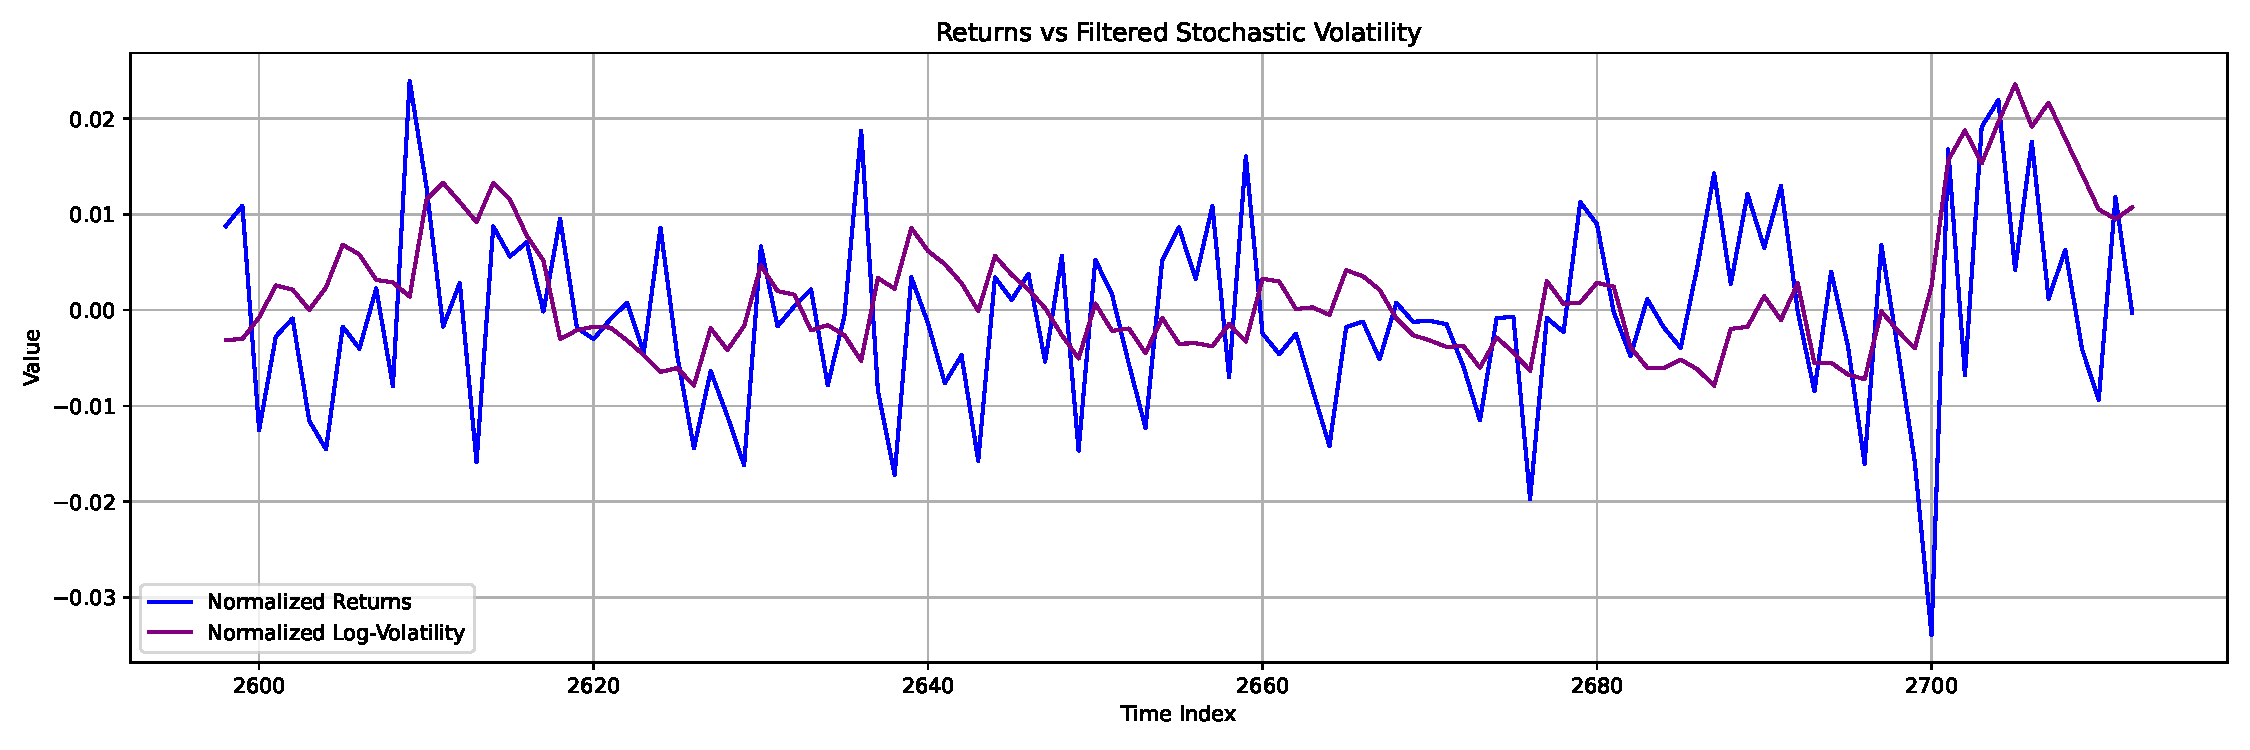
\includegraphics[width=\textwidth]{Images/stochastic_volatility.pdf}
    \caption{Normalized actual returns vs filtered log-volatility (Stochastic Volatility Model).}
    \label{fig:sv_actual_vs_pred}
\end{figure}

\begin{figure}[h!]
    \centering
    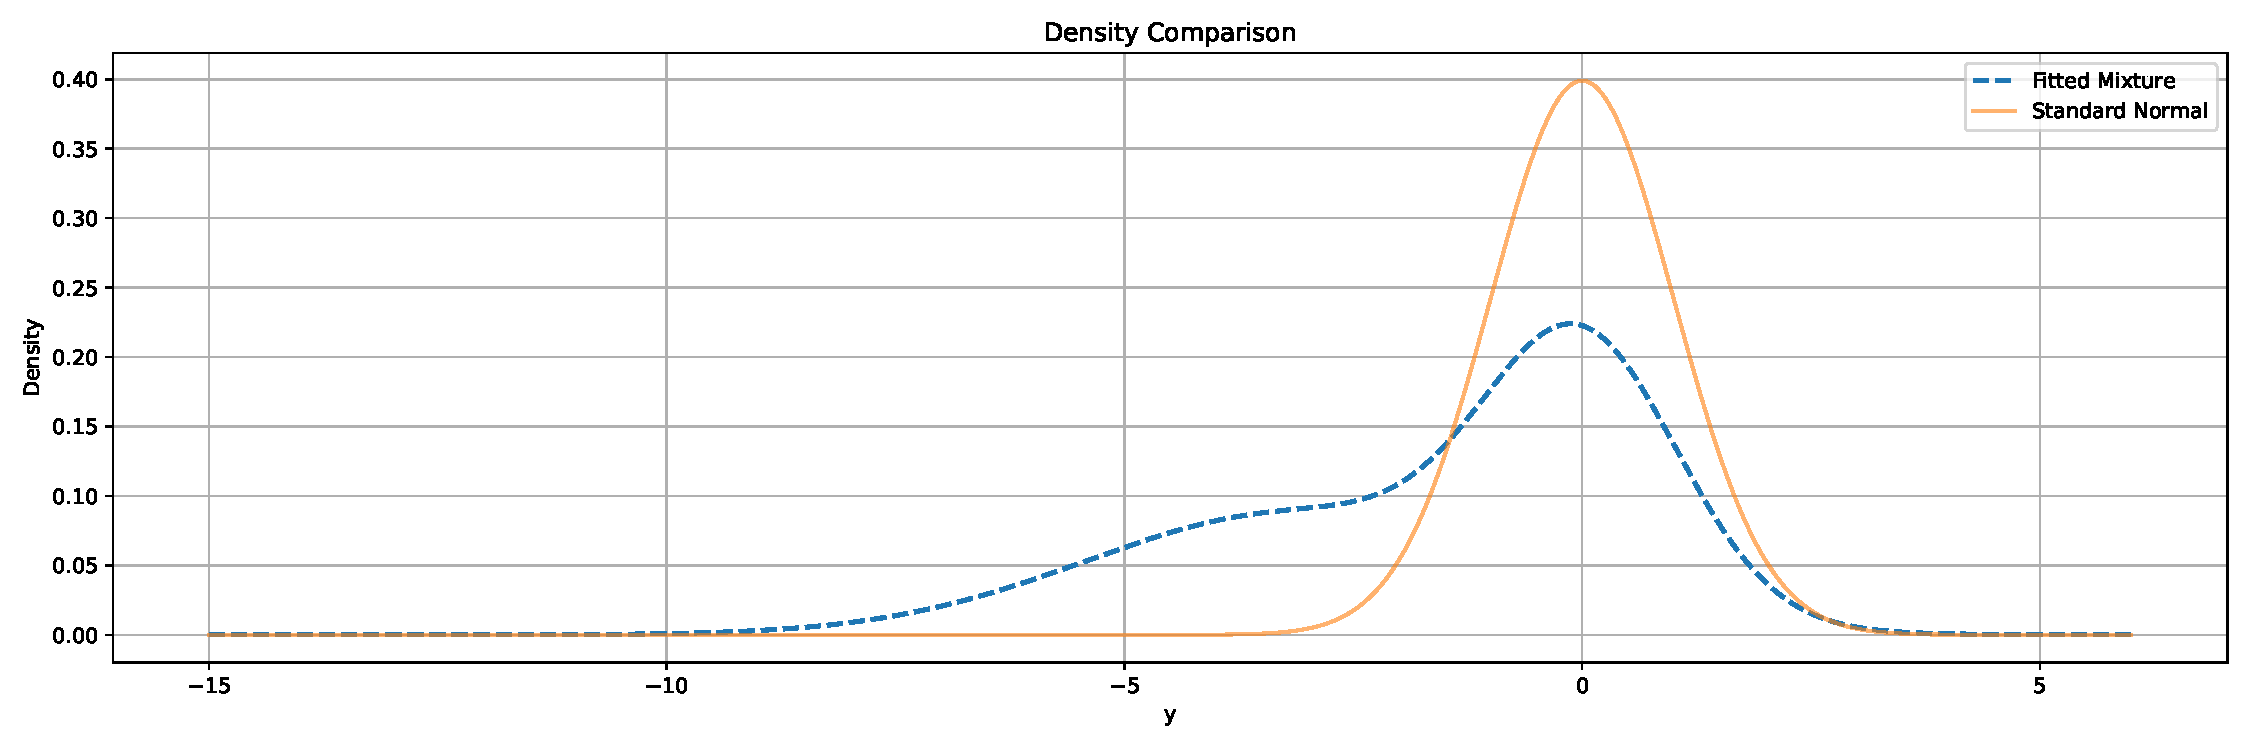
\includegraphics[width=\textwidth]{Images/stochastic_volatility_density.pdf}
    \caption{Density comparison of actual returns vs fitted returns (Stochastic Volatility Model).}
    \label{fig:sv_density}
\end{figure}

\section{Ensemble Learning Results}
\subsection{Actual vs Predicted Returns}
Figure~\ref{fig:ensemble_actual_vs_pred} presents the predicted daily returns from the ensemble meta-learner compared with the actual close returns.

\subsection{Performance Metrics}
\begin{itemize}
    \item \textbf{RMSE:} 0.0064
    \item \textbf{R\textsuperscript{2} Score:} ----
\end{itemize}

\begin{figure}[h!]
    \centering
    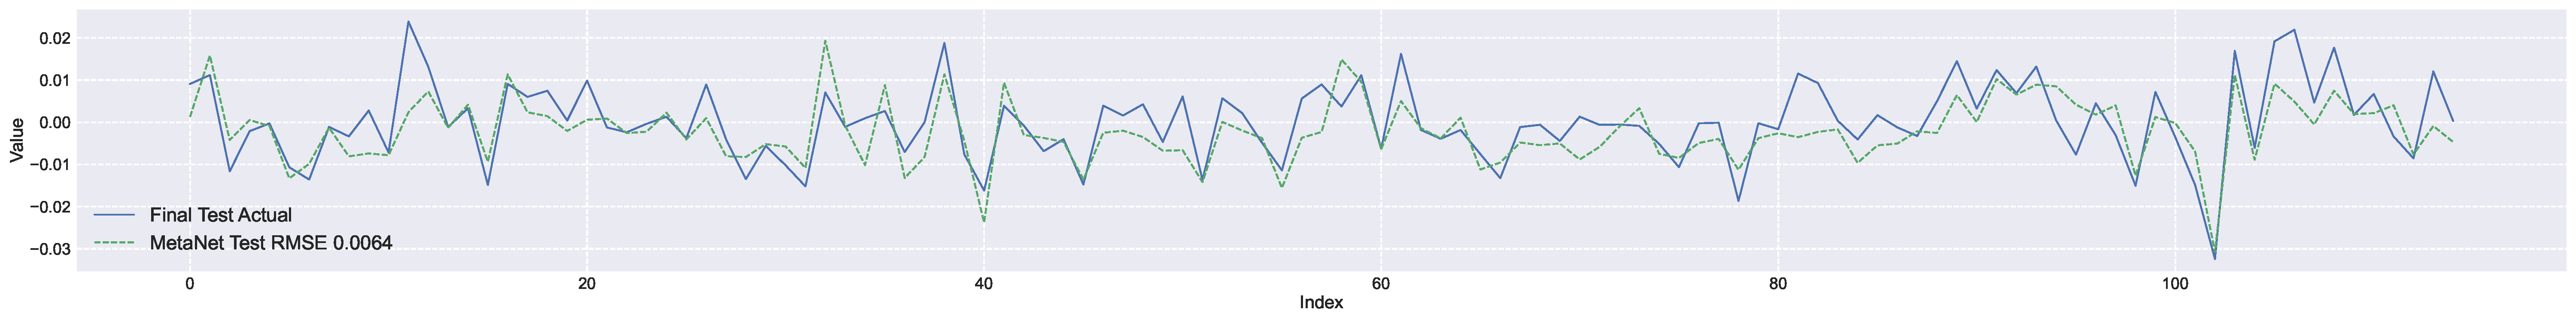
\includegraphics[width=\textwidth]{Images/metanet_final_test_plot_s.pdf}
    \caption{Actual vs Predicted daily close return (Ensemble Meta-Learner).}
    \label{fig:ensemble_actual_vs_pred}
\end{figure}

\section{Transformer GAN Results}
\subsection{Actual vs Predicted Returns}
Figure~\ref{fig:tgan_actual_vs_pred} illustrates the ability of the Transformer-based GAN to replicate daily return dynamics.

\subsection{Performance Metrics}
\begin{itemize}
    \item \textbf{RMSE:} ----
    \item \textbf{R\textsuperscript{2} Score:} ----
\end{itemize}

\begin{figure}[h!]
    \centering
    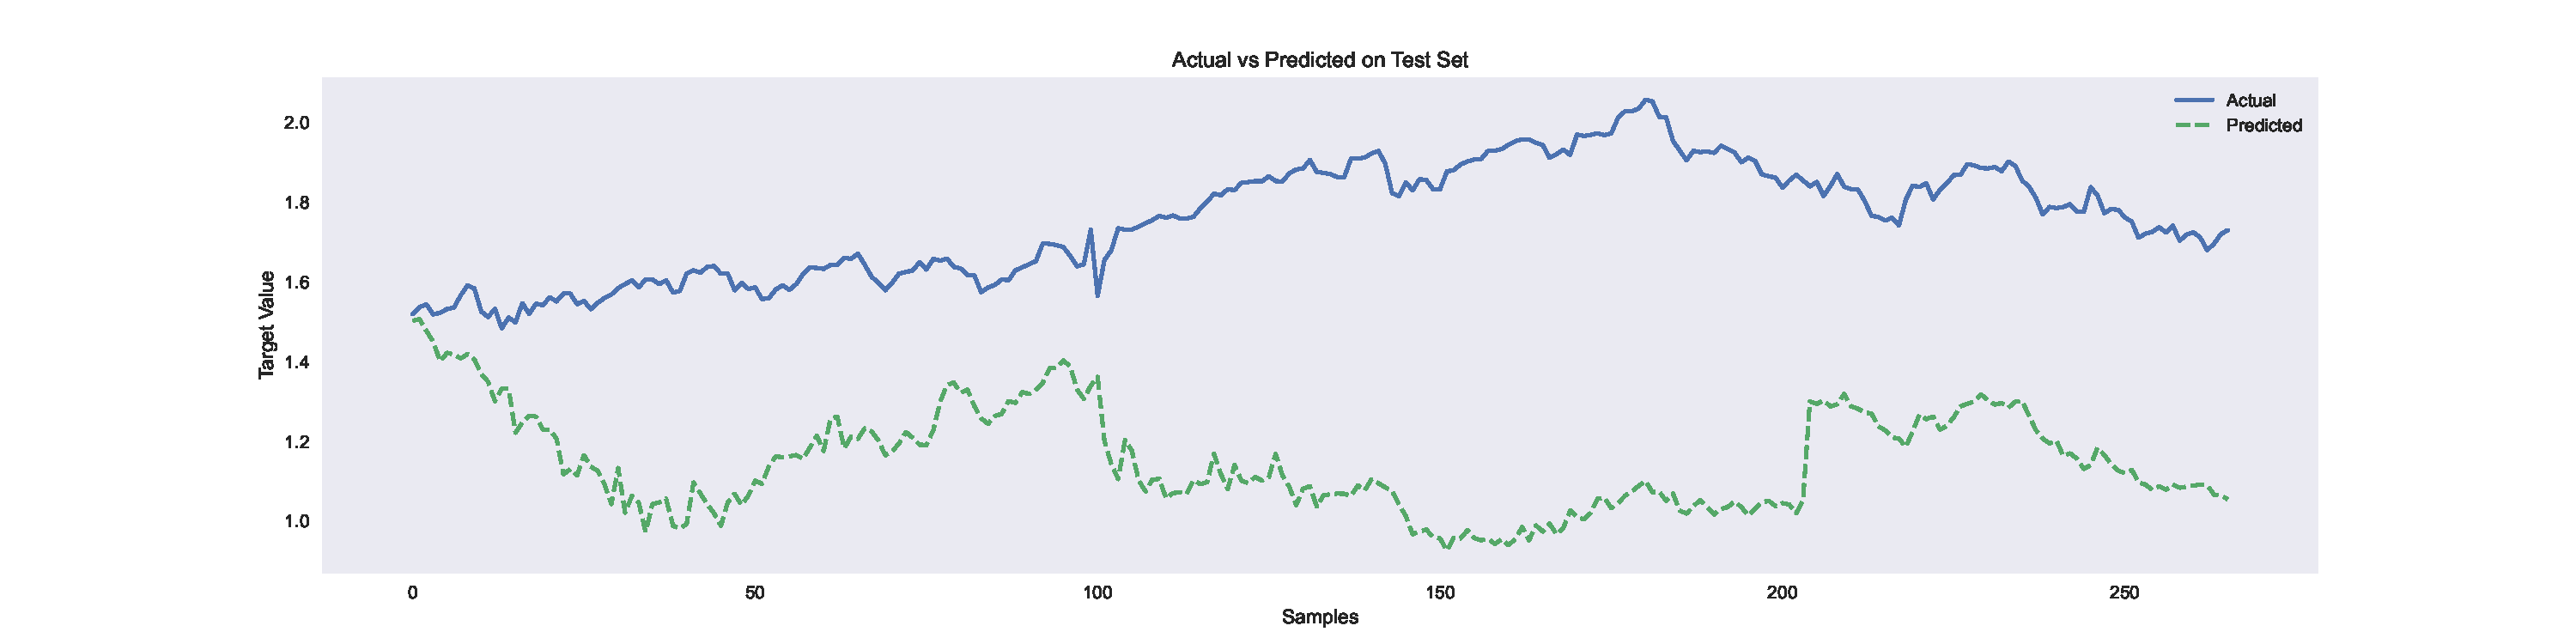
\includegraphics[width=\textwidth]{Images/_8_ActualVsPred_c.pdf}
    \caption{Actual vs Predicted daily close return (Transformer GAN).}
    \label{fig:tgan_actual_vs_pred}
\end{figure}

\section{RAGIC Framework Results}
\subsection{Actual vs Predicted Returns}
Figure~\ref{fig:ragic_actual_vs_pred} compares the predicted returns from the RAGIC framework against the actual returns, reflecting the model’s interpretability and precision.

\subsection{Performance Metrics}
\begin{itemize}
    \item \textbf{RMSE:} ----
    \item \textbf{R\textsuperscript{2} Score:} ----
\end{itemize}

\begin{figure}[h!]
    \centering
    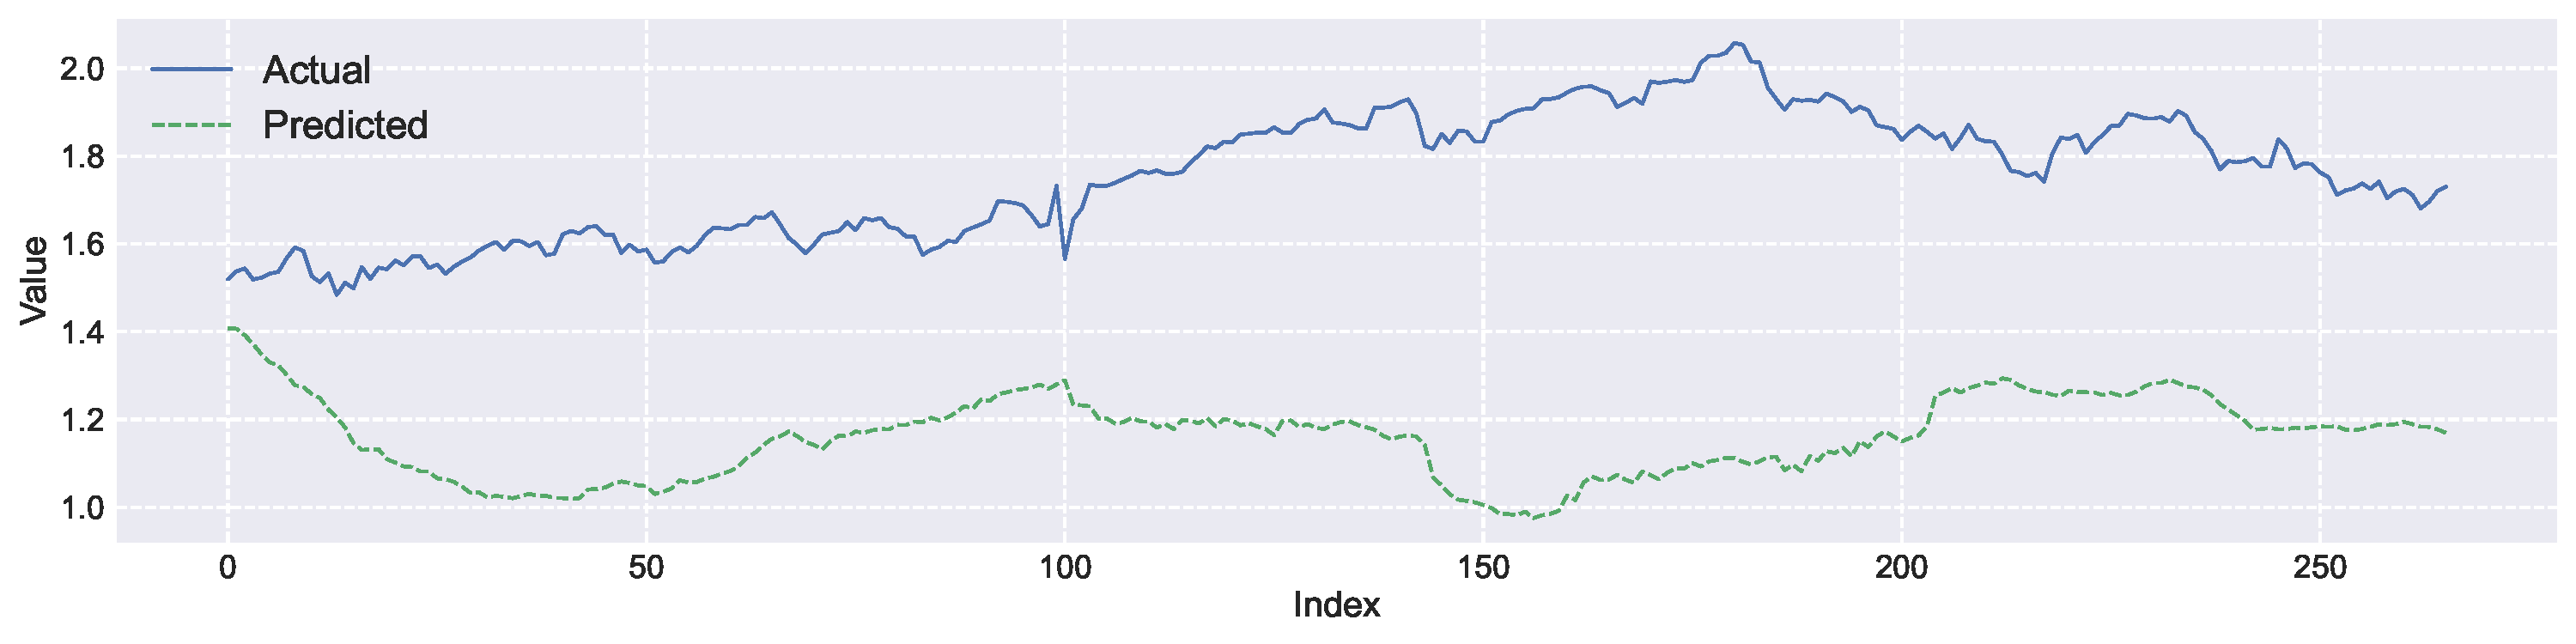
\includegraphics[width=\textwidth]{Images/9_Act_vs_Pred_Point.pdf}
    \caption{Actual vs Predicted daily close return (RAGIC Framework).}
    \label{fig:ragic_actual_vs_pred}
\end{figure}

